% \levelC{Dataset}
This study uses the Govdocs1 dataset \cite{garfinkel_bringing_2009}, which was fully downloaded and its files were grouped by extension. This dataset has files with 63 different extensions. The 33 extensions with less than 200 files were discarded. From the remaining 30 extensions, listed in table \ref{tab:govdocs1}, 200 files of each were randomly selected, 100 to use in the training dataset and 100 to use in the validation dataset.

\begin{table}[!ht]
    \centering
    \caption{Govdocs1 dataset}
    \label{tab:govdocs1}
\begin{tabular}{|l|l|l|}
\hline
Extension & Number of files & Number of blocks \\ \hline
                                                  \hline
pdf       & 231232          & 268071071    \\ \hline
html      & 214568          & 25710908     \\ \hline
jpg       & 109233          & 73242253     \\ \hline
txt       & 78286           & 99435540     \\ \hline
doc       & 76616           & 60654930     \\ \hline
xls       & 62635           & 58718224     \\ \hline
ppt       & 49702           & 251210471    \\ \hline
gif       & 36302           & 5962516      \\ \hline
xml       & 33458           & 16954875     \\ \hline
ps        & 22015           & 56547464     \\ \hline
csv       & 18360           & 6843009      \\ \hline
gz        & 13725           & 17748905     \\ \hline
log       & 9976            & 8467819      \\ \hline
eps       & 5191            & 5756138      \\ \hline
% unk       & 5186            & 2983922      \\ \hline
png       & 4125            & 2207489      \\ \hline
swf       & 3476            & 3798321      \\ \hline
dbase3    & 2601            & 38972        \\ \hline
pps       & 1619            & 7432480      \\ \hline
rtf       & 1125            & 958239       \\ \hline
kml       & 993             & 309422       \\ \hline
kmz       & 943             & 549462       \\ \hline
% text      & 839             & 1527118      \\ \hline
hlp       & 659             & 8692         \\ \hline
f         & 602             & 94543        \\ \hline
sql       & 462             & 244634       \\ \hline
wp        & 364             & 87643        \\ \hline
dwf       & 299             & 85500        \\ \hline
java      & 292             & 14530        \\ \hline
pptx      & 215             & 1151796      \\ \hline
% fits      & 182             & 678128       \\ \hline
% tmp       & 180             & 28426        \\ \hline
% tex       & 163             & 10520        \\ \hline
% docx      & 163             & 65969        \\ \hline
% troff     & 110             & 8020         \\ \hline
% bmp       & 72              & 62686        \\ \hline
% sgml      & 62              & 44138        \\ \hline
% gls       & 60              & 517          \\ \hline
% pub       & 55              & 1421         \\ \hline
% xlsx      & 37              & 12910        \\ \hline
% fm        & 25              & 6717         \\ \hline
% zip       & 10              & 31525        \\ \hline
% ttf       & 10              & 1540         \\ \hline
% xbm       & 8               & 578          \\ \hline
% wk1       & 7               & 6493         \\ \hline
% sys       & 7               & 15           \\ \hline
% ileaf     & 4               & 1656         \\ \hline
% exported  & 3               & 324          \\ \hline
% data      & 3               & 1733         \\ \hline
% odp       & 2               & 2384         \\ \hline
% mac       & 2               & 0            \\ \hline
% lnk       & 2               & 2            \\ \hline
% js        & 2               & 36           \\ \hline
% g3        & 2               & 498          \\ \hline
% chp       & 2               & 73           \\ \hline
% 123       & 2               & 434          \\ \hline
% wk3       & 1               & 229          \\ \hline
% vrml      & 1               & 660          \\ \hline
% squeak    & 1               & 25354        \\ \hline
% py        & 1               & 480          \\ \hline
% pst       & 1               & 20           \\ \hline
% icns      & 1               & 0            \\ \hline
% bin       & 1               & 7            \\ \hline
\end{tabular}
\end{table}


% \levelC{Hardware}
The experiments did not take advantage of GPU acceleration and were  conducted on a single computer with 256GB of RAM and with 2 Intel\textregistered Xeon\textregistered E5-2630 v2 processors, with 6 cores each, with 2 hyper-threads per core, or 24 hyper-threads in total. 


% \levelC{Software}
The main softwares and frameworks used to build the experiments were Python 3.6, Jupyter notebook, Tensorflow 1.14.0, Keras 2.2.4-tf, and Fedora Linux 27.

% repository
The source code for the experiments is available at \url{http://github.com/atilaromero/ML}.
\todo[inline]{create a cleaner repository just for the paper}

Section \ref{sec:evalmodels} evaluates some alternative models in the file fragment classification task. The expectation was to identify the most promising models for improvement. Instead, an apparent limit was found on how far these models could be improved. 

Section \ref{sec:numberofclasses} describes how does the accuracy of neural network models change relative to the number of classes. It was observed that a high accuracy in the file fragment classification task could be achieved only when the number of classes was small. Also, when compared with each other, file types with high entropy data showed the lowest accuracy values.

Section \ref{sec:exprandom} investigates the hypothesis that some part of these errors may be explained by the inability of the models to distinguish high entropy data from random data. The portion of data that could be identified as not random was higher than expected. While some of errors could have the explanation mentioned in the hypothesis, it could only explain about 1/3 of the observed errors (16.5\% out of 55
\%) \todo{revise numbers}.

\levelB{Exploratory research of models based on accuracy}
\label{sec:evalmodels}

\levelC{Objective}
In this exploratory research, different neural networks are trained and validated
at the file fragment identification task. Their accuracy is then compared,
to identify which models should be considered or disregarded in the remaining phases.


\levelC{Sampling}
To select a sample instance from the Govdocs1 dataset, first a random file is selected among those available, without replacement. Then, a block from this file is randomly selected. After all files have participated in the process, the process may be repeated as long as necessary. This way, all files are considered and the classes are easily balanced.
This contrasts with the sampling technique applied in other works, where all the sectors are grouped together before sampling, which may lead to a imbalance between classes.

\levelC{Inputs}
%one-hot
The input features of the network for each instance is a 512x256 matrix representing only one block of 512 bytes of a random file of the dataset. Each of the 512 bytes is one-hot encoded, meaning that its value is converted into a vector with 256 elements, with only one of them set to 1, corresponding to the value of the byte, while the others are set to zero. A batch size of 100 was used, with 30 steps per epoch. \todo{remake with 28 after excluding text and unk?}

%8bits
% The input features of the network for each instance is a 512x8 matrix representing only one block of 512 bytes of a random file of the dataset. Each of the 512 bytes uses a custom encoding where each of the 8 bits of a byte is represented as -1 or 1, depending whether the bit is 0 or 1. During initial tests, this encoding was compared to three other encodings: one-hot encoding, 8 bits represented as 0 or 1\todo{include citation}, and 8 bits represented as [0,1] and [1,0] \cite{hiester_file_2018}. More research should be done in the future to determine the best of the four, but initial results suggest they have similar impact on the model accuracy. The one-hot encoding has the disadvantage of increasing the input matrix size by a factor of 32.

\levelC{Outputs}
The output of the network for a given instance is a vector with a size equal to the number of classes, subjected to a softmax function, which applies the exponential function on the vector and then normalizes it. Each value will represent the predicted probability that the instance belongs to a specific class.


\levelC{Models}
The networks under consideration used different combinations of convolutional, max pooling, LSTM, and fully connected layers,
%loss
applying categorical crossentropy as the loss function. Binary crossentropy and mean squared error were considered during initial tests, but categorical crossentropy gave faster training times.

Fourteen models participated in this evaluation. One of then is a simple single layer perceptron. Two of them use LSTM layers without convolutional layers, while 3 of them use convolutional layers without LSTM layers. Eight models combine convolutional layers and LSTM layers. Table \ref{tab:models} outline the parameters of the models, which can be analysed in more details in the code repository \todo{repository}. The convolutional layers do not use padding. 

\newcommand{\paint}{\cellcolor{gray!25}}
\begin{table}[!ht]
    \centering
    \footnotesize
    \caption{14 models trained on 30 classes}
    \label{tab:models}
\begin{tabular}{l||l|l|l||l|l|l||l|l||l}
\hline
Model  & \multicolumn{3}{l||}{Convolutional layers} & \multicolumn{3}{l||}{Max pooling} & \multicolumn{2}{l||}{LSTM} & Dense  \\ \hline
       & output       & window       & stride      & pool    & stride    & channel    & output     & return       & output \\ 
       & size         & size         & length      & size    & length    & first      & size       & sequences    & size   \\ \hline
                                                                                                                              \hline
D      & \paint       & \paint       &     \paint  & \paint  &  \paint   & \paint     & \paint     & \paint       & 30     \\ \hline
LD     & \paint       & \paint       &     \paint  & \paint  &  \paint   & \paint     & 32         & no           & 30     \\ \hline
LL     & \paint       & \paint       &     \paint  & \paint  &  \paint   & \paint     & 32         & yes          & \paint \\ 
       & \paint       & \paint       &     \paint  & \paint  &  \paint   & \paint     & 32         & no           & \paint \\ \hline
CD     & 64           & 64           & 8           & \paint  &  \paint   & \paint     & \paint     & \paint       & 30     \\ \hline
CM     & 30           & 32           & 1           & 481     & 1         & no         &  \paint    & \paint       & \paint \\ \hline
CCM    & 30           & 32           & 1           &         &           &            & \paint     & \paint       & \paint \\ 
       & 30           & 2            & 2           & 240     & 1         & no         & \paint     & \paint       & \paint \\ \hline
CL     & 30           & 32           & 32          & \paint  &  \paint   & \paint     & 30         & no           & \paint \\ \hline
CML    & 32           & 32           & 32          & 2       & 2         & yes        & 30         & no           & \paint \\ \hline
CLL    & 32           & 32           & 32          & \paint  &  \paint   & \paint     & 64         & yes          & \paint \\ 
       &              &              &             & \paint  &  \paint   & \paint     & 30         & no           & \paint \\ \hline
CLD    & 256          & 16           & 16          & \paint  &  \paint   & \paint     & 128        & no           & 30     \\ \hline
CCL    & 128          & 8            & 8           & \paint  &  \paint   & \paint     &            &              & \paint \\ 
       & 64           & 8            & 8           & \paint  &  \paint   & \paint     & 30         & no           & \paint \\ \hline
CCLL   & 128          & 8            & 8           & \paint  &  \paint   & \paint     & 64         & yes          & \paint \\ 
       & 64           & 8            & 8           & \paint  &  \paint   & \paint     & 30         & no           & \paint \\ \hline
CMCML  & 128          & 8            & 8           & 2       & 2         & yes        &            &              & \paint \\ 
       & 64           & 8            & 8           & 2       & 2         & yes        & 30         & no           & \paint \\ \hline
CMCMLL & 128          & 8            & 8           & 2       & 2         & yes        & 64         & yes          & \paint \\ 
       & 64           & 8            & 8           & 2       & 2         & yes        & 30         & no           & \paint \\ \hline
\end{tabular}
\end{table}

%optimization
All the trainings use the Adam \cite{kingma_adam:_2014}
optimization algorithm to guide backpropagation, which was selected because it performed well in the preliminary results without fine tuning of parameters.

% Constraints
The models where trained until no further improvement was observed in the last 60 epochs.

\levelC{Results}
%exp18
The two models that used LSTM layers without convolutional layers presented a slower learning in comparison with the others, as can be seen in figure \ref{fig:learning}. The validation accuracy values can be consulted in figure \ref{fig:models}.

\noindent
\begin{figure*}[htb!]
\centering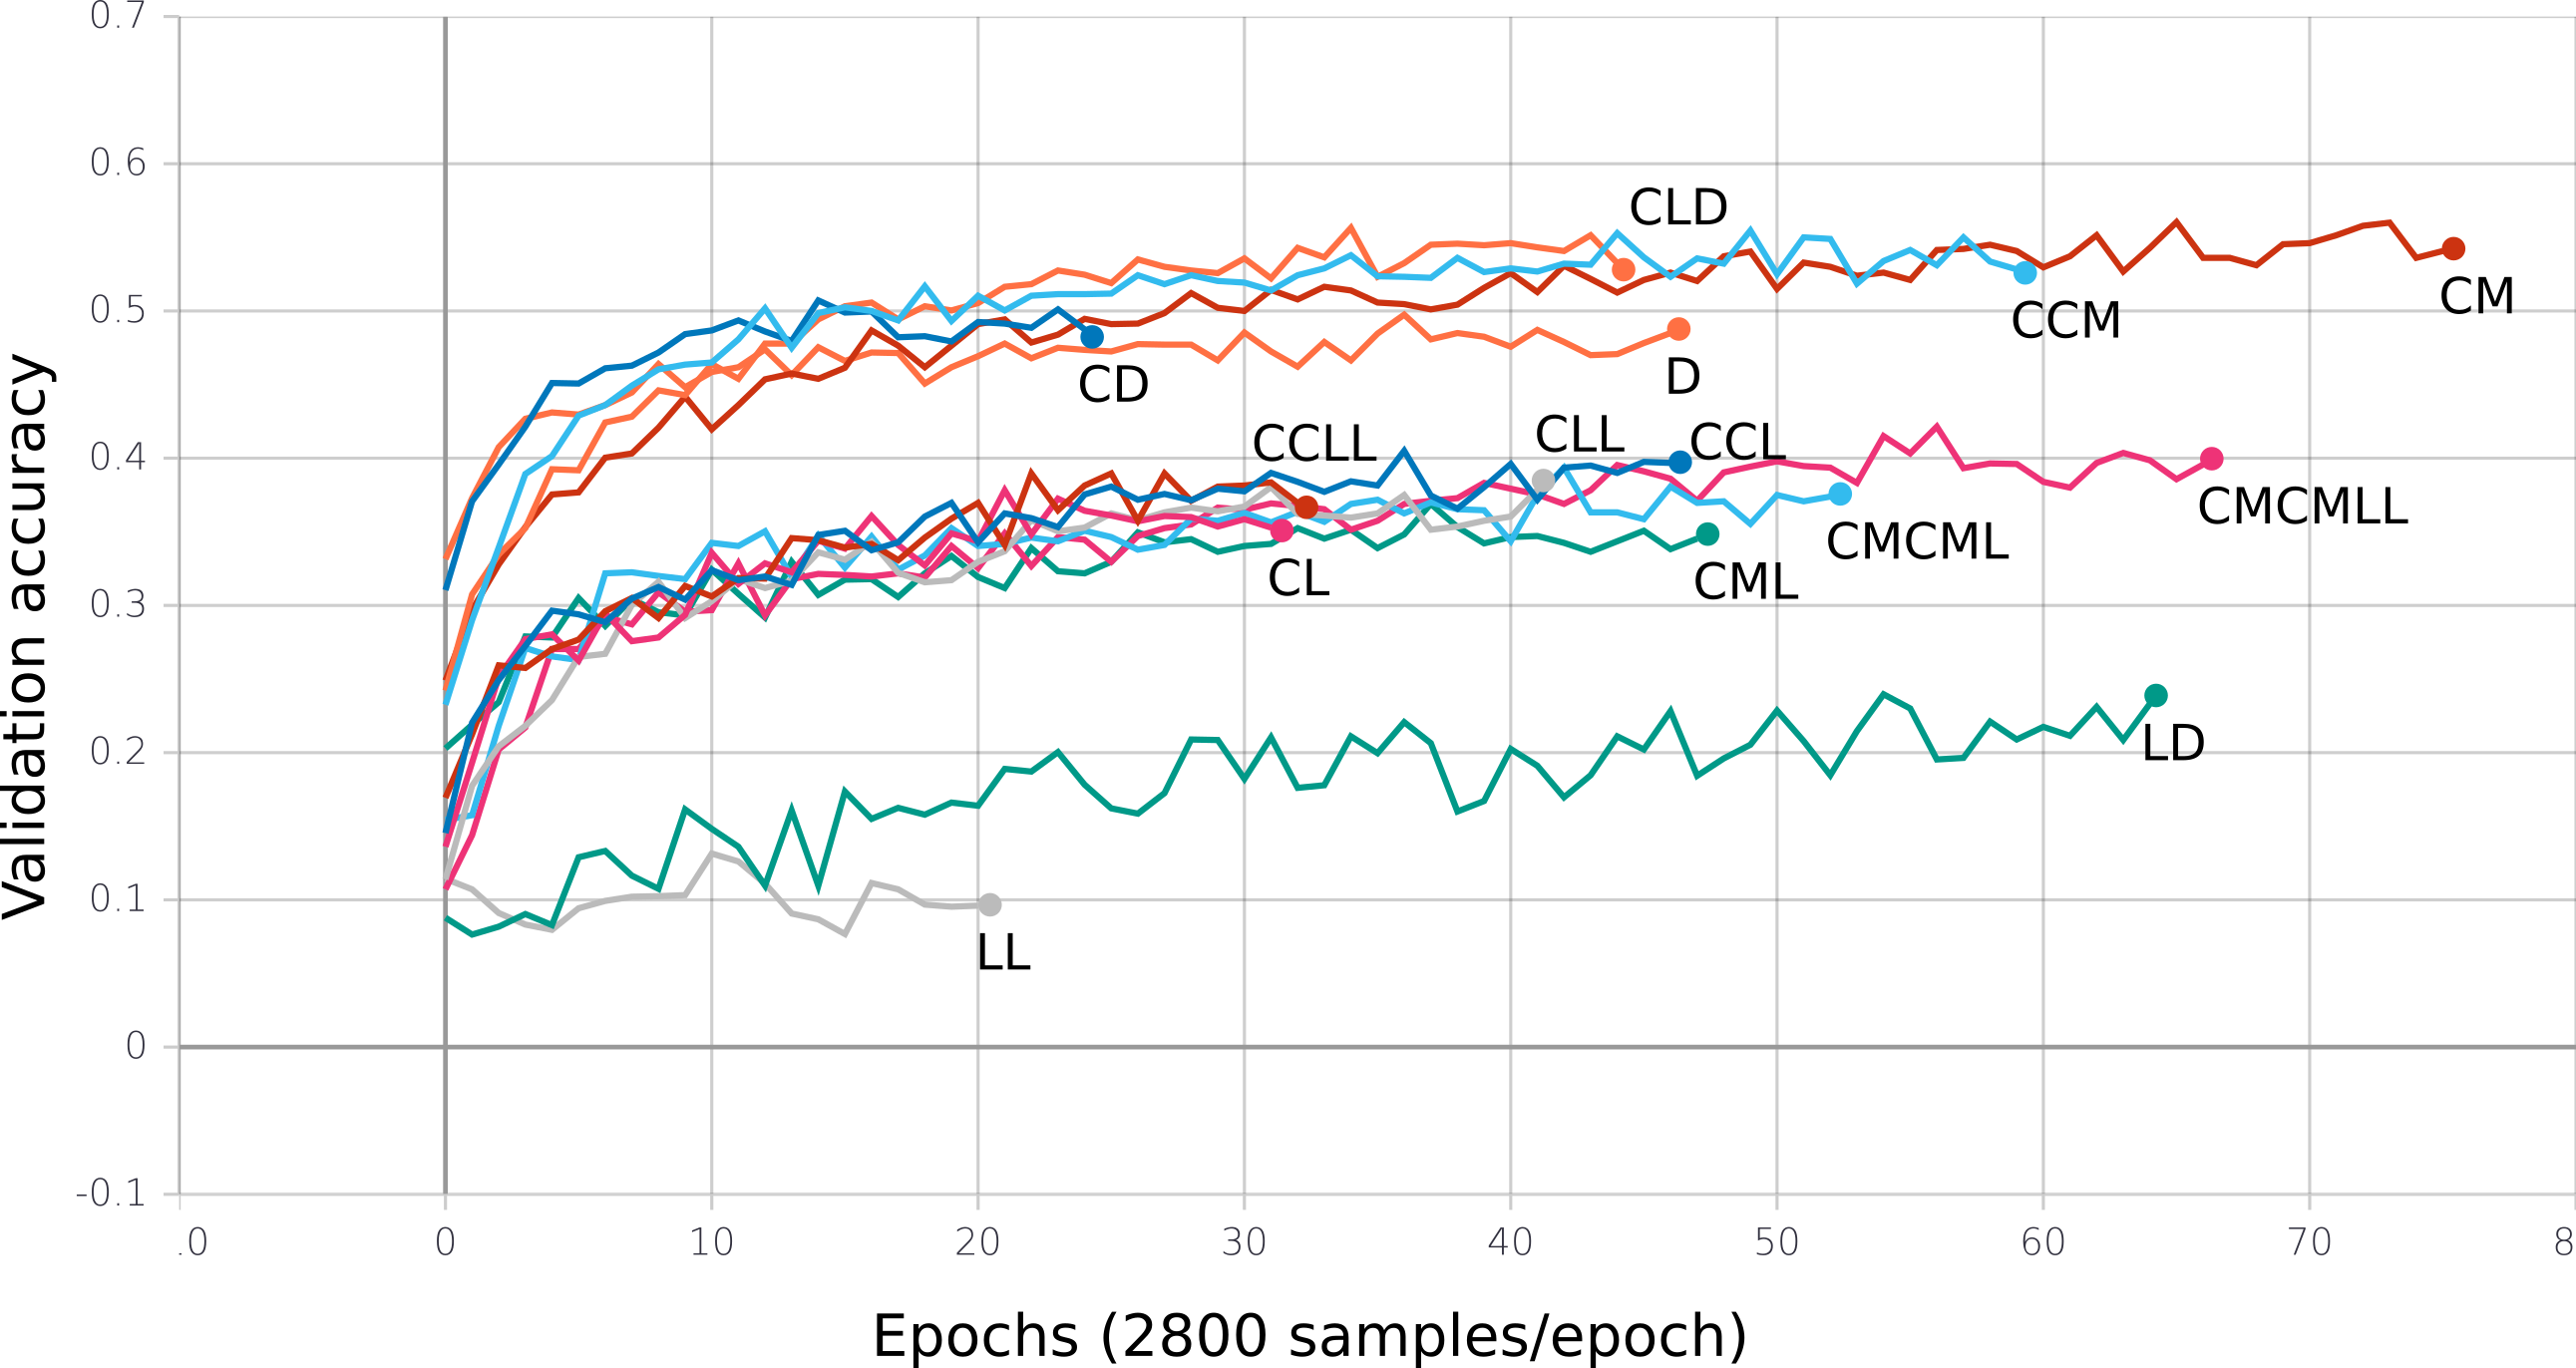
\includegraphics[width=1.0\textwidth]{content/epoch_val_categorical_accuracy.png}
\caption{\label{fig:learning}Learning curves of some models (validation accuracy vs. time)}%
\end{figure*}

\noindent
\begin{figure*}[htb!]
\centering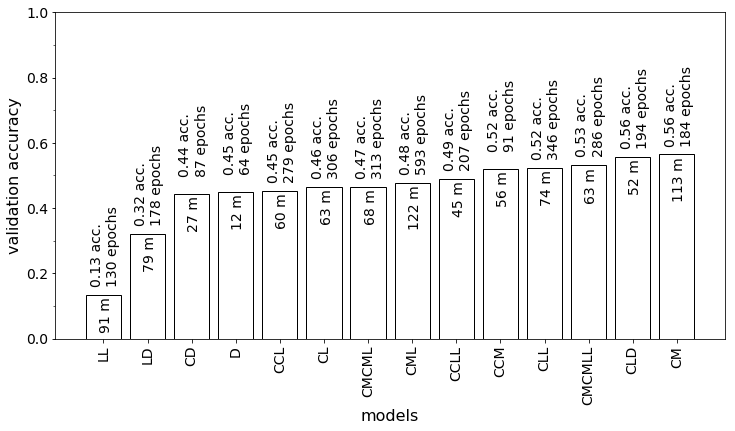
\includegraphics[width=1.0\textwidth]{content/models.png}
\caption{\label{fig:models}The bar plot shows the validation accuracy of the considered models. Their training time, in minutes, and the total epochs processed is also indicated. The training was halted when no further improvement was observed for 60 consecutive epochs.)}%
\end{figure*}



The remaining models after ten minutes already showed signs of being close to their limit.
Their accuracy results were in the 0.44-0.56 range.

The selected model for further research, identified as ``CLD'', achieved an accuracy of 0.56.

To check if the two slower models could give better result if executed for a longer period, they were trained for 10 hours. The model identified as ``LD'', which uses a LSTM layer followed by a fully connected layer, was able to achieve 0.494 accuracy, while the other, ``LL'', achieved only 0.153.



%stagnation in learning with such short times, combined with low final accuracy suggests that the dataset present some patterns that are easily recognizable, while the rest of the dataset present a very hard classification task.

% \levelC{Limitations and threats to validity}
In this exploratory research, the models were not trained until exhaustion. This was initially done to identify which models would be most promising for future testing, but further attempts to tune layer types, quantity and parameters were insufficient to raise accuracy above the 0.44-0.56 range, which suggests that selection or tuning of models may not be best approach to improve results.





\levelB{Descriptive research on influence of number of classes}
\label{sec:numberofclasses}
\levelC{Objective}
In the previous section, it was observed that achieving 0.6 accuracy on file fragment classification using 28 classes was a difficult task to the considered models. In other studies results \cite{hiester_file_2018} \cite{sportiello_context-based_2012} \cite{amirani_feature-based_2013} \cite{maslim_distributed_2014} and on initial tests, the achieved accuracy for small number of classes was considerably higher. Hiester \cite{hiester_file_2018}, for instance, achieves an accuracy of 98\% using four classes.

This section investigates how does the accuracy of the considered models change in relation to the number of classes in the dataset.


\levelC{Dataset}
Several independent models were trained with 2 to 28 extensions from the Govdocs1 dataset. For each number in the range 2 to 28, a random subset of extensions was selected to compose the dataset. Each extension has 200 file samples, half placed in the training dataset and half in the validation dataset. Each dataset was used to train a new model, that should distinguish between the selected subset of extensions in that filtered dataset. This process was repeated five times.



In addition to this sampling of extensions using different quantities of classes, all 378 combinations of pairs of extensions were compared. Each pair was used to compose a dataset and to train a new model for each one, using the same process described in the previous paragraph.

\levelC{Models}
The same sampling, input, and output details described in section \ref{sec:evalmodels} were used here. The model identified as ``CM'' was selected to be used.

\levelC{Results}
% decrease in accuracy
Figure \ref{fig:nclasses} shows the graph of accuracy versus number of classes for the ``CM'' model. The bottom line indicates, for comparison, what the accuracy would be for a random guessing classifier. An increase in the number of classes appears to be  correlated with a decrease in accuracy. Another relevant aspect of the graph is that the range of the results seems to be smaller when more classes are used.  

This pattern is understandable: as the number of classes grows, the harder the classification problem is, leading to a decrease in accuracy, while the individual contributions of each class to the overall result diminishes, leading to an increase in precision.

This behavior is an important aspect to consider during the evaluation of file fragments studies. As Beebe et al. \cite{beebe_sceadan:_2013} have mentioned, studies that select fewer classes tend to yield higher results. 

Still, with 46\% \todo{check} of samples being misclassified when the number of classes is 28, the question of what are the error sources and how they can be addressed requires attention.

\noindent
\begin{figure*}[htb!]
\centering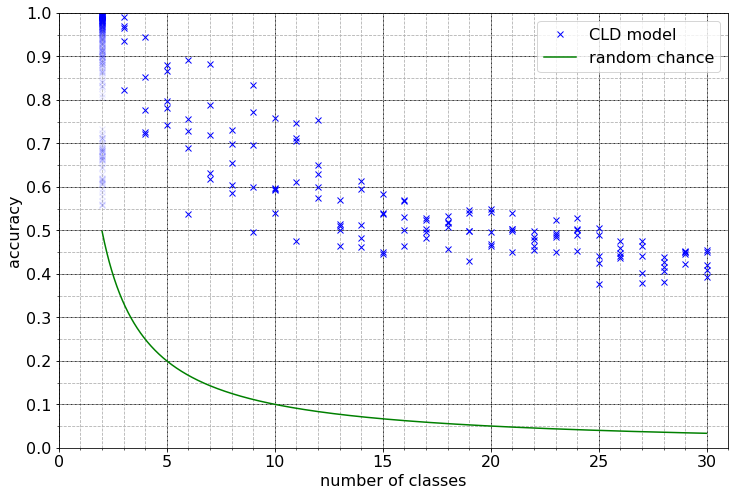
\includegraphics[width=1.0\textwidth]{content/nclasses.png}
\caption{\label{fig:nclasses}Validation accuracy by number of classes}%
\end{figure*}

Figure \ref{fig:dual} shows the graph of the accuracy of each class when compared individually with each one of the others. Generally, file types with higher entropy tend to have lower minima, with the GIF \todo{check} file type being a notable exception. Most of these files use some form of compression, like image files for example. 


\noindent
\begin{figure*}[htb!]
\centering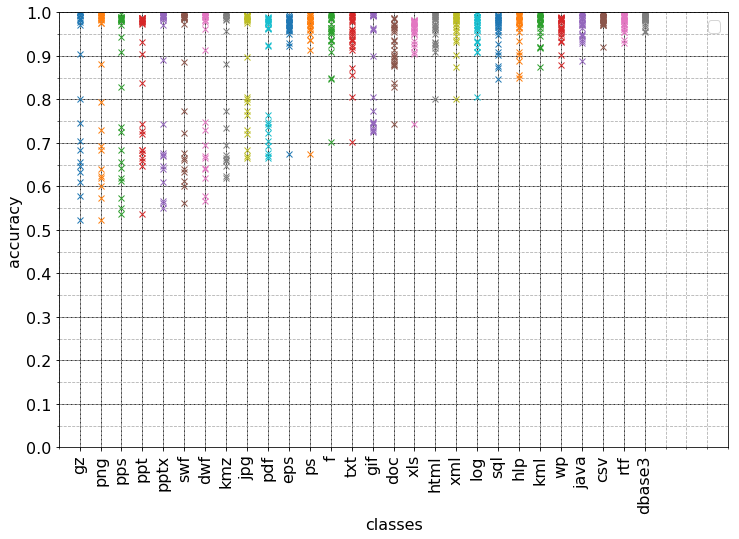
\includegraphics[width=1.0\textwidth]{content/dual.png}
\caption{\label{fig:dual}Validation accuracy of models trained with pair of classes}%
\end{figure*}


The accuracy obtained after the training of models with pairs of classes was used to build a 28x28 matrix, using 0.5 in the main diagonal entries. This number was chosen because a pair of indistinguishable classes would have this accuracy on average. Then, a Principal Component Analysis (PCA) \cite{amirani_new_2008} was used to treat this matrix. The result is shown in figures \ref{fig:pca} and \ref{fig:pca2}. Again some file types with high entropy emerge as a promising group, \todo{check} ``dwf'',
``jpg'',
``pps'',
``ppt'',
``gz'',
``png'',
``pptx'',
``swf'',
``kmz'',
and ``pdf''.

\noindent
\begin{figure*}[htb!]
\centering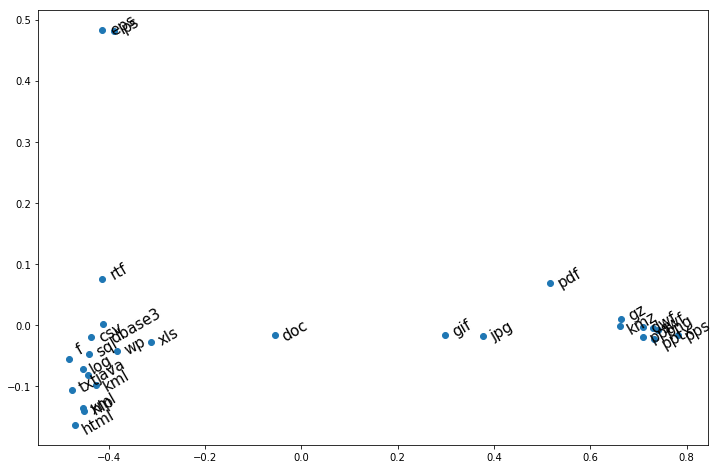
\includegraphics[width=1.0\textwidth]{content/pca.png}
\caption{\label{fig:pca}PCA of accuracy of models trained with pair of classes}%
\end{figure*}


\noindent
\begin{figure*}[htb!]
\centering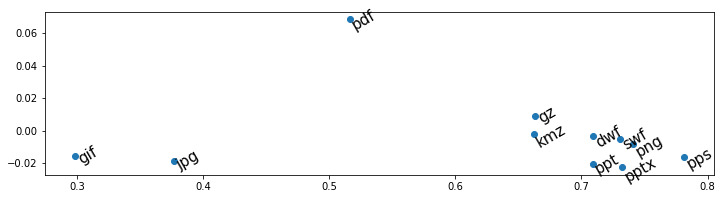
\includegraphics[width=1.0\textwidth]{content/pca2.png}
\caption{\label{fig:pca2}PCA of accuracy of models trained with pair of classes - detail}%
\end{figure*}


% the problem of unseen file types
% \levelC{Limitations and threats to validity}


\levelB{Experiment on random data detection}

